\documentclass[a4paper,12pt]{article}
\usepackage[utf8]{inputenc}
\usepackage{graphicx}
\graphicspath{ {./imgs/} }
\usepackage{fancyhdr} % For headers and footers
\usepackage{geometry}
\usepackage{hyperref} % For clickable links
\usepackage{longtable} % For long tables that can span multiple pages
\usepackage{array}     % For better column formatting

% Adjust margins
\geometry{
    top=4cm, 
    bottom=2.5cm, 
    left=2.5cm, 
    right=2.5cm,
    headheight=3cm, % Ensures sufficient space for header content
    headsep=0.5cm,
    }

% Define the custom headers
\fancypagestyle{firstpage}{% First page header style
    \fancyhf{} % Clear all header/footer fields
    \fancyhead[L]{%
        
\includegraphics[height=1.5cm]{heig_logo.png} \\
    }
    \fancyhead[R]{%
        
\includegraphics[height=1.5cm]{reds_logo.png} \\
    }
    \fancyfoot{} % No footer on the first page
}

% Define other pages style
\fancypagestyle{otherpages}{%
    \fancyhf{}
    \fancyhead[L]{%
        
\includegraphics[height=1.5cm]{heig_logo.png} \\
    }
    \fancyhead[R]{%
        \small Laboratoire 6: Mesure du temps de réaction \\
        Rodrigo Lopez Dos Santos / Urs Behrmann \\
    }
    \fancyfoot[C]{\small page \thepage}
}

\author{Rodrigo Lopez Dos Santos, Urs Behrmann}

\setlength{\parskip}{1em} % Définit un espace entre chaque paragraphe
\setlength{\parindent}{0pt} % Optionnel : enlève l'indentation des paragraphes

\begin{document}

\emergencystretch=1em % Ajoute une flexibilité d'espacement

% First page content
\thispagestyle{firstpage}


\vspace*{2cm}
\begin{center}
    \Huge Laboratoire 6 \\
    \vspace{0.2cm}
    \Large Mesure du temps de réaction\\
    \vspace{1cm}
    \small Départements : TIC\\
    Unité d'enseignement ARE\\
\end{center}

\vspace{9cm}

\renewcommand{\arraystretch}{1.5} % Adjust row height

\begin{flushleft} % Left-align the table
    \begin{tabular}{@{}l l@{}}
        \textbf{Auteurs :}       & \textbf{Rodrigo Lopez Dos Santos} \\
                                 & \textbf{Urs Behrmann} \\
        \textbf{Professeur :}    & \textbf{Etienne Messerli} \\
        \textbf{Assistant :}     & \textbf{Anthony Convers} \\
        \textbf{Classe :}        & \textbf{ARE} \\
        \textbf{Salle de labo :} & \textbf{A07} \\
        \textbf{Date :}          & \textbf{27.01.2025} \\
    \end{tabular}
\end{flushleft}

\newpage

% Apply the other pages style
\pagestyle{otherpages}

\tableofcontents

\newpage

% Content for subsequent pages
\section{Introduction}

\break

\section{Analyse et conception}

\subsection{Plan d'adressage}

\begin{longtable}{|p{4cm}|p{5cm}|p{6cm}|}
    \hline
    \textbf{Address (offset)} & \textbf{Read}             & \textbf{Write}         \\
    \hline
    \endfirsthead
    \hline
    \textbf{Address (offset)} & \textbf{Read}             & \textbf{Write}         \\
    \hline
    \endhead
    \hline
    \endfoot
    \hline
    \endlastfoot

    0x00                      & [31..0] Interface user ID & reserved               \\
    \hline
    0x04                      & [31..4] "0..0"            & reserved               \\
                              & [3..0] buttons            &                        \\
    \hline
    0x08                      & [31..10] "0..0"           & reserved               \\
                              & [9..0] switches           &                        \\
    \hline
    0x0C                      & [31..10] "0..0"           & [31..10] reserved      \\
                              & [9..0] leds               & [9..0] leds            \\
    \hline
    0x10                      & [31..28] reserved         & [31..28] reserved      \\
                              & [27..21] hex3             & [27..21] hex3          \\
                              & [20..14] hex2             & [20..14] hex2          \\
                              & [13..7] hex1              & [13..7] hex1           \\
                              & [6..0] hex0               & [6..0] hex0            \\
    \hline
    0x14                      & [31..2] reserved          & [31..1] reserved       \\
                              & [1] interrupt             & [0] clear interrupt    \\
                              & [0] statut flanc montant  &                        \\
    \hline
    0x18                      & [31..1] reserved          & [31..1] reserved       \\
                              & [0] interrupt mask        & [0] set interrupt mask \\
    \hline
    0x1C                      & [31..1] reserved          & [31..0] reserved       \\
                              & [0] Max10 status          &                        \\
    \hline
    0x20                      & [31..0] reserved          & [31..0] reserved       \\
                              & [0] Max10 busy            &                        \\
    \hline
    0x24                      & [31..0] reserved          & [31..1] reserved       \\
                              &                           & [0] Max10 CS           \\
    \hline
    0x28                      & [31..0] reserved          & [31..0] reserved       \\
                              &                           & [0] Max10 data         \\
    \hline
    0x2C                      & [31..0] reserved          & [31..0] reserved       \\
                              &                           & [0] Counter start      \\
    \hline
    0x30                      & [31..0] reserved          & [31..0] reserved       \\
                              &                           & [0] Counter stop       \\
    \hline
    0x34                      & [31..0] reserved          & [31..0] reserved       \\
                              & [0] Counter delta         &                        \\
    \hline
    0x38                      & [31..0] reserved          & [31..0] reserved       \\
                              & [0] Counter error         &                        \\
    \hline
    0x3C                      & [31..0] reserved          & [31..0] reserved       \\
                              & [0] Counter cycle count   &                        \\
    \hline
\end{longtable}

\subsection{Emetteur série asynchrone}

Pour l'émetteur série asynchrone, nous avons dû utilsé une baudrate de 9600. Mais la vitesse de l'horloge étant de 50 MHz, nous avons dû utiliser un timer pour diviser cette fréquence. Nous avons donc utilisé un timer qui compte jusqu'à 5208 pour obtenir une fréquence de environ 9600 Hz.

\break

\section{Interface (VHDL)}

\subsection{Schéma}

\includegraphics[width=\textwidth]{are_labo6_schéma.png}

\break

\subsubsection{Composants}

\textbf{counter\_cycle.vhd}

Implémente un compteur cyclique utilisé pour mesurer des périodes définies, probablement à 20 ns de précision.

\textbf{counter\_reaction.vhd}

Spécifique à la mesure du temps de réaction, il démarre et arrête le comptage en fonction des signaux d’entrée.

\textbf{counter\_setpoint.vhd}

Permet de définir un seuil ou un point d'arrêt pour le comptage.

\textbf{serial\_async\_transmitter.vhd}

Implémente l'émetteur série asynchrone de 20 bits, sans parité, pour communiquer avec la carte Max10\_leds.
Prend en charge le protocole spécifié (bit de départ, 20 bits de données, bit d'arrêt).

\subsubsection{Processus}

\textbf{write\_outputs}

Gère les sorties des LEDs et des afficheurs 7 segments (HEX) en écrivant les données reçues depuis le bus Avalon.

\textbf{read\_address\_decoder}

Décode les adresses Avalon pour diriger les lectures vers les périphériques appropriés, comme les boutons et interrupteurs.

\textbf{write\_interrupt}

Permet de masquer, activer ou acquitter les interruptions générées par KEY0, en interagissant avec les registres d'interruption.

\textbf{read\_interrupt\_source}

Renvoie l'état des interruptions et des détections de flanc pour une gestion correcte des signaux.

\break

\textbf{sync\_inputs}

Synchronise les entrées des boutons et interrupteurs pour garantir leur stabilité face aux métastabilités.

\textbf{write\_max10}

Prend en charge la conversion des données pour les transmettre à la carte Max10\_leds via l'émetteur série.

\textbf{write\_cnt\_spt}

Permet de configurer le seuil du compteur `cnt\_spt` et de démarrer ou arrêter son fonctionnement en fonction des besoins.

\textbf{read\_data\_to\_bus}

Lit les données des registres internes (par exemple, valeurs des compteurs ou état des périphériques) et les transmet via le bus Avalon pour qu'elles soient accessibles au processeur.

\break

\section{Programme (C)}

\subsection{fichiers \& utilisation}

\subsubsection{UART (uart.c / uart.h)}

\begin{itemize}
    \item Fournit des fonctions pour configurer et gérer la communication série (baudrate, envoi de messages, gestion FIFO).
    \item Utilisé pour afficher des messages dans un terminal distant via UART.
\end{itemize}

\subsubsection{Interruptions (exceptions.c / exceptions.h)}

\begin{itemize}
    \item Configure le contrôleur générique d’interruptions (GIC).
    \item Définit les vecteurs d’exceptions pour gérer des interruptions (notamment pour le bouton KEY0).
    \item Gère l'interruption principale avec la fonction fpga\_ISR.
\end{itemize}

\subsubsection{}

\begin{itemize}
    \item Avalon (avalon.h, avalon\_functions.c / avalon\_functions.h)
    \item Encapsule l’accès au bus Avalon pour interagir avec les registres des périphériques (LEDs, switches, afficheurs).
    \item Fournit des macros de lecture/écriture pour manipuler les données efficacement.
\end{itemize}

\subsubsection{Application principale (app.c / app.h)}

\begin{itemize}
    \item Implémente la logique du jeu en utilisant une machine à états :
    \item Initialisation (APP\_INIT).
    \item Attente (APP\_WAIT).
    \item Début du jeu (APP\_START\_GAME).
    \item Erreur (APP\_ERROR).
    \item Gère les entrées (boutons, interrupteurs) et affiche les résultats sur l’UART et les LEDs.
    \item Implémente l'ISR de la FPGA (KEY0), ISR utilisé pour la gestion de fin de jeu lorsqu'une jeu est commencé (APP\_START\_GAME)
\end{itemize}

\subsection{Logique principale}

L'objectif du programme est de mesurer le temps de réaction de l'utilisateur en utilisant les composants de la carte DE1-SoC et MAX10. Voici la logique étape par étape :

\subsubsection{Initialisation}

\begin{itemize}
    \item Configure l’UART, le GIC, et les périphériques via Avalon.
    \item Désactive les interruptions jusqu'à ce que l'application soit prête.
    \item Affiche les instructions utilisateur sur l’UART.
\end{itemize}

\subsubsection{Machine à états}

\begin{itemize}
    \item APP\_INIT : Configure les LEDs, afficheurs, et active les interruptions.
    \item APP\_WAIT : Surveille les entrées utilisateur (boutons, interrupteurs) pour déterminer l’état suivant.
    \item APP\_START\_GAME : Affiche le symbole de début et démarre le compteur.
    \item APP\_INIT\_GAME : Configure un temps aléatoire pour démarrer la mesure.
    \item APP\_ERROR : Gère les erreurs (ex. : configuration invalide de la carte MAX10).
\end{itemize}

\subsubsection{Gestion des interruptions}

\begin{itemize}
    \item Lorsqu'un utilisateur appuie sur KEY0, une interruption déclenche :
    \item Le calcul du temps de réaction via un compteur.
    \item L’affichage des résultats (UART, LEDs, HEX).
    \item La mise à jour des statistiques (meilleur/pire temps, erreurs, essais).
\end{itemize}

\subsubsection{Affichage des résultats :}

\begin{itemize}
    \item Les afficheurs HEX montrent les données (dernier temps, meilleures performances, erreurs, essais) selon la configuration choisie via SW0 à SW3.
    \item L’UART fournit un résumé complet des performances.
\end{itemize}

\break

\section{Tests}

\subsection{Simulation (interface)}

\subsubsection{IOs}

On a fait une première simulation pour vérifier les IOs. On a fait une suite de R/W sur les adresses de la mémoire. On a vérifié que les valeurs lues correspondaient aux valeurs écrites.

\begin{center}
    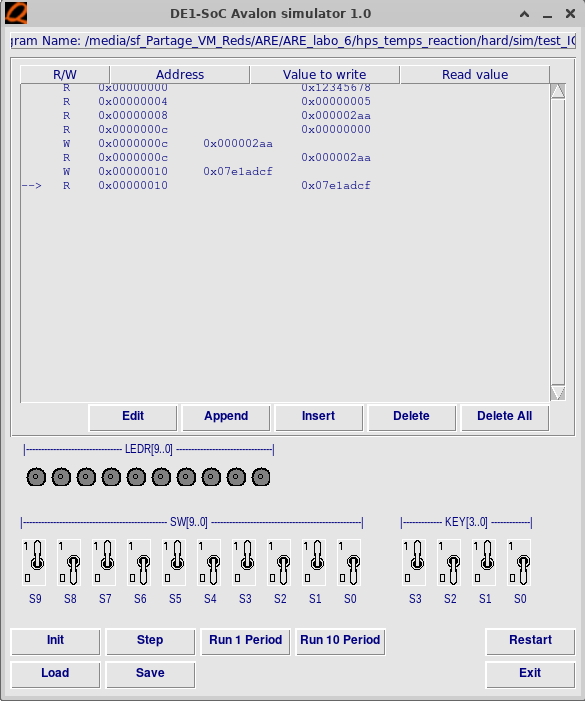
\includegraphics[width=300px]{test_IOs.png}
\end{center}

\break

\subsubsection{Compteurs}

On a fait une deuxième simulation pour vérifier le compteur. On a fait un test avec 0 périodes supplémentaires. On voit bien que le compteur s'incrémente de 2 avec chaque instruction. On a un total de 6 périodes. entre le début et la fin du comptage.

\begin{center}
    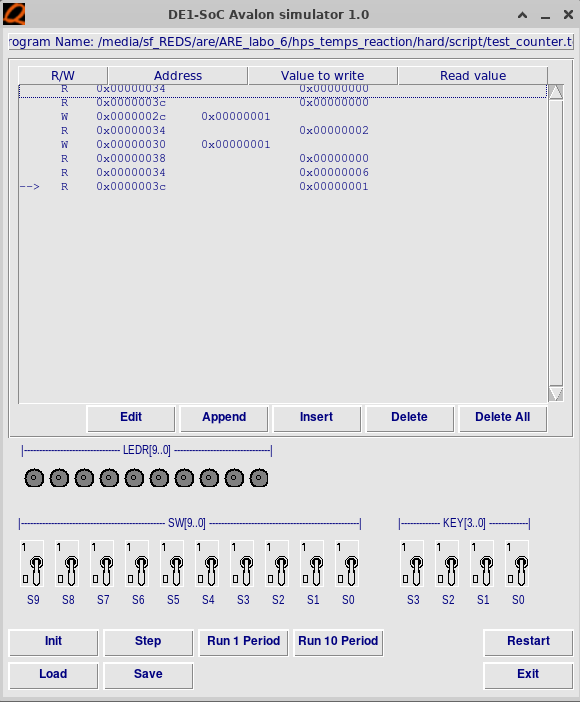
\includegraphics[width=300px]{test_cmpt_0_periods.png}
\end{center}

Avec 10 périodes supplémentaires, on voit qu'on a un total de 16 périodes entre le début et la fin du comptage.

\begin{center}
    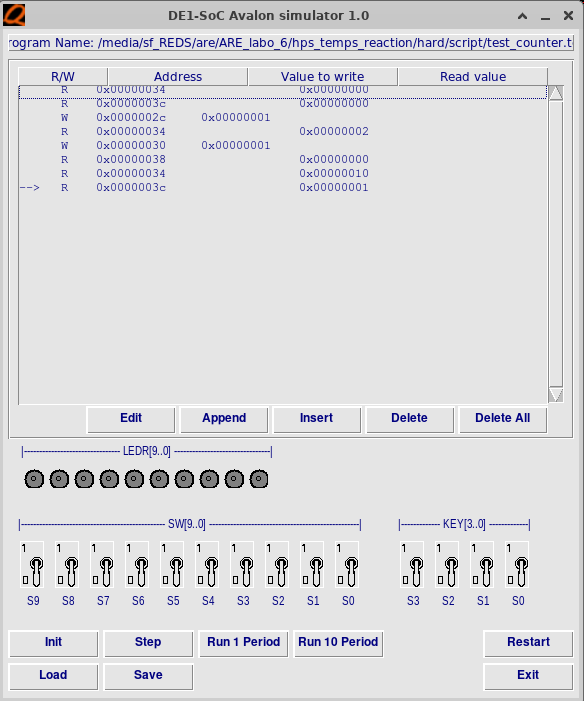
\includegraphics[width=300px]{test_cmpt_10_periods.png}
\end{center}

\break

\subsubsection{Interruptions}

Pour les interruptions, on a fait un premier test pour vérifier que l'interruption se déclenche bien. On a changé la position du bouton 0 de 0 à 1. On voit bien que l'interruption se déclenche.

On peut bien voir qu'on n'a pas d'interruption à la première lecture du registre 0x14 et qu'on a une interruption à la deuxième lecture.

Dans la deuxième partie de la simulation, on a activé le masque d'interruption. On voit bien que l'interruption ne se déclenche pas, mais que le bit d'indication de flanc montant est à 1.

\begin{center}
    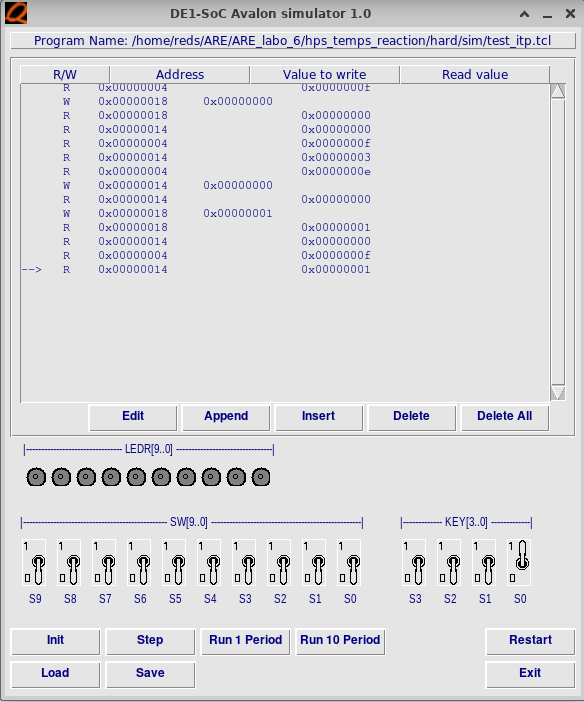
\includegraphics[width=300px]{test_itp.png}
\end{center}

\break

\subsubsection{Test serial transmission to max10}

Pour tester la transmission série vers le max10, on a fait un test avec une valeur de 0xabaa et un chip select de 0x01. Cela nous donne une data de 0x01abaa ou bien 0b0001\_1010\_1011\_1010\_1010.

On a aussi changé la vitesse de la baudrate pour avoir une pulse tous les 4 cycles. 

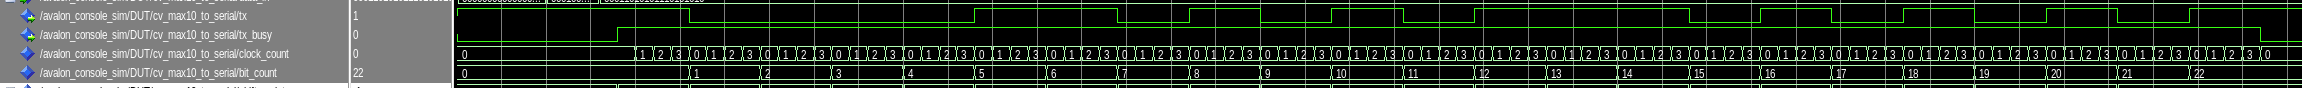
\includegraphics[width=\textwidth]{test_max10.png}

\break

\subsection{Visuel via UART (Programme)}

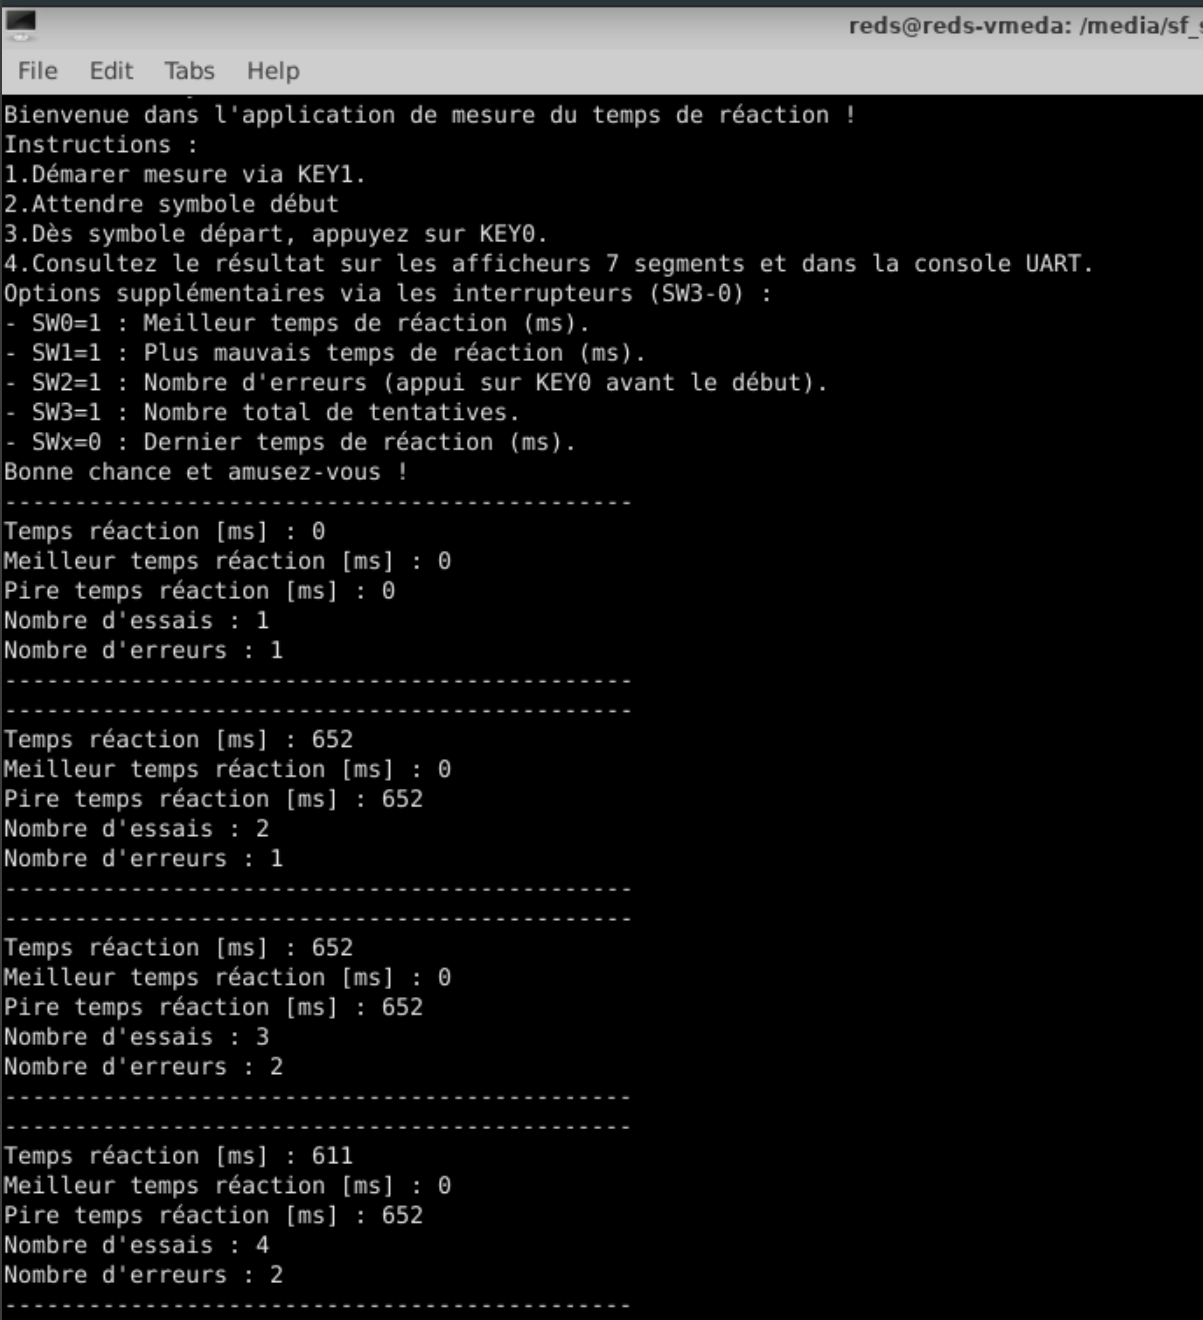
\includegraphics[width=\textwidth]{tests_via_uart.png}

\break

\section{Conclusion}
Le projet a permis de développer une application fonctionnelle respectant les exigences du cahier des charges, malgré des défis rencontrés tout au long de sa réalisation. Voici une synthèse des principaux points :

\subsection{Points marquants et réussites}

\begin{itemize}
    \item Conformité au cahier des charges : Toutes les fonctionnalités spécifiées, comme la gestion des LEDs, les afficheurs 7 segments, la communication série avec la MAX10 et la mesure du temps de réaction, ont été implémentées et validées.
    \item Code C complet et fonctionnel : La logique de l'application est robuste et a permis de gérer les différents états du système tout en intégrant efficacement les interruptions, les entrées utilisateur et les affichages.
    \item Gestion des aléas : Un problème d'allumage aléatoire des LEDs de la MAX10 a été corrigé grâce à un "patch" introduisant une attente de 1 ms entre chaque envoi, garantissant ainsi un comportement stable.
    \item Approche modulaire : La séparation claire entre le VHDL et le C a facilité l'intégration et le dépannage des différentes parties.
\end{itemize}

\subsection{Défis rencontrés et axes d'amélioration}

\begin{itemize}
    \item Communication série initiale : Une première conception imprécise pour la communication série avec la MAX10 a entraîné des retards importants (2 à 3 semaines) en raison d'une phase de débogage prolongée. Cela a limité le temps disponible pour perfectionner le projet.
    \item Problèmes liés au VHDL : Certains comportements inattendus, comme l'interruption déclenchée au démarrage ou le problème d'allumage des LEDs, semblent liés à des lacunes dans notre conception VHDL. Une version non finalisée du fichier avl\_user\_interface\_not\_finished.vhdl est incluse, illustrant nos efforts pour améliorer cette partie, bien que non testée faute de temps.
    \item Pression temporelle : Les dernières semaines ont été marquées par un rythme intense, limitant nos capacités à itérer sur certaines solutions et à approfondir les tests.
\end{itemize}

\subsection{Bilan global}

Malgré ces défis, nous sommes fiers de présenter une solution fonctionnelle. Bien qu'elle ne soit pas exempte de limitations, elle répond aux attentes principales du laboratoire et démontre notre capacité à surmonter des obstacles complexes dans un délai restreint. Ce projet nous a permis de renforcer nos compétences en conception embarquée, en gestion des interruptions, et en communication série.

\vspace{2cm}
\noindent
\textbf{Date:} 27.01.25 \\
\textbf{Noms des étudiants:} \textit{Rodrigo Lopez Dos Santos, Urs Behrmann}

\break

\section{Annexe}


\end{document}